% ============================================================================
%  Interview presentation, Mobile Perception Systems Lab, TU Eindhoven
%  Richard Cernansky
%  Compile with: latexmk -pdf main.tex   (pdflatex, two runs for frame totals)
% ============================================================================
\documentclass[aspectratio=169,11pt,t]{beamer}

\usepackage[utf8]{inputenc}
\usepackage[T1]{fontenc}
\usepackage[english]{babel}
\usepackage{lmodern}
\usepackage{booktabs}
\usepackage{amsmath,amssymb}
\usepackage{xcolor}
\usepackage{csquotes}
\usepackage{tikz}
\usetikzlibrary{positioning,arrows.meta,calc}

% Bibliography: the thesis bibliography, copied into bib/references.bib.
% Build with: latexmk -pdf main.tex   (runs biber automatically)
\usepackage[backend=biber,style=numeric,sorting=none,maxnames=2,
            minnames=1,giveninits=true,doi=false,isbn=false,url=false]{biblatex}
\addbibresource{bib/references.bib}
\setbeamertemplate{bibliography item}[text]
\renewcommand*{\bibfont}{\scriptsize}
% Cite marks on slides stay small and out of the way
\newcommand{\refcite}[1]{\textcolor{tuered}{\scriptsize\cite{#1}}}

% ----------------------------------------------------------------------------
%  Classical beamer look: rounded shadowed blocks, section bar, info footline
% ----------------------------------------------------------------------------
\useinnertheme[shadow=true]{rounded}
\useoutertheme[subsection=false]{smoothbars}
\usecolortheme{whale}
\usecolortheme{orchid}
\setbeamertemplate{navigation symbols}{}

% ----------------------------------------------------------------------------
%  TU/e colour scheme.  TU/e corporate red is the single brand colour here,
%  every other shade is derived from it.  Swap the one hex value below if the
%  official brand guide differs.
% ----------------------------------------------------------------------------
\definecolor{tuered}{HTML}{C81919}
\definecolor{tuedark}{HTML}{3C3C3B}
\definecolor{tuelight}{HTML}{F7EDED}

\setbeamercolor{structure}{fg=tuered}
\setbeamercolor{normal text}{fg=tuedark}
\setbeamercolor{alerted text}{fg=tuered}

\setbeamercolor{palette primary}{bg=tuered,fg=white}
\setbeamercolor{palette secondary}{bg=tuered!80!black,fg=white}
\setbeamercolor{palette tertiary}{bg=tuered!60!black,fg=white}
\setbeamercolor{palette quaternary}{bg=tuedark,fg=white}

\setbeamercolor{titlelike}{parent=palette primary}
\setbeamercolor{frametitle}{bg=tuered,fg=white}
\setbeamercolor{section in head/foot}{bg=tuered!80!black,fg=white}
\setbeamercolor{author in head/foot}{bg=tuered!60!black,fg=white}
\setbeamercolor{title in head/foot}{bg=tuered,fg=white}
\setbeamercolor{date in head/foot}{bg=tuered!60!black,fg=white}

\setbeamercolor{block title}{bg=tuered,fg=white}
\setbeamercolor{block body}{bg=tuelight,fg=tuedark}
\setbeamercolor{block title alerted}{bg=tuered!65!black,fg=white}
\setbeamercolor{block body alerted}{bg=tuelight,fg=tuedark}
\setbeamercolor{block title example}{bg=tuedark,fg=white}
\setbeamercolor{block body example}{bg=tuedark!8,fg=tuedark}

\setbeamercolor{itemize item}{fg=tuered}
\setbeamercolor{itemize subitem}{fg=tuered!70}
\setbeamercolor{enumerate item}{fg=tuered}
\setbeamercolor{description item}{fg=tuered}

\setbeamerfont{frametitle}{series=\bfseries}
\setbeamerfont{block title}{size=\small,series=\bfseries}
\setbeamerfont{description item}{series=\bfseries}

% Classic three-box info footline
\setbeamertemplate{footline}{%
  \leavevmode%
  \hbox{%
    \begin{beamercolorbox}[wd=.30\paperwidth,ht=2.4ex,dp=1.1ex,leftskip=.3cm,rightskip=.3cm]{author in head/foot}%
      \usebeamerfont{author in head/foot}\insertshortauthor
    \end{beamercolorbox}%
    \begin{beamercolorbox}[wd=.54\paperwidth,ht=2.4ex,dp=1.1ex,leftskip=.3cm,rightskip=.3cm]{title in head/foot}%
      \usebeamerfont{title in head/foot}\insertshorttitle
    \end{beamercolorbox}%
    \begin{beamercolorbox}[wd=.16\paperwidth,ht=2.4ex,dp=1.1ex,leftskip=.3cm,rightskip=.3cm plus1fil]{date in head/foot}%
      \usebeamerfont{date in head/foot}\hfill\insertframenumber\,/\,\inserttotalframenumber
    \end{beamercolorbox}%
  }%
  \vskip0pt%
}

% ----------------------------------------------------------------------------
%  Shorthands
% ----------------------------------------------------------------------------
\newcommand{\up}{$\uparrow$}
\newcommand{\dn}{$\downarrow$}
\newcommand{\tueemph}[1]{{\color{tuered}\textbf{#1}}}
% Shrink a box to \textwidth if it is wider, never enlarge it
\newcommand{\fitwidth}[1]{%
  \resizebox{\ifdim\width>\textwidth \textwidth\else \width\fi}{!}{#1}}

\tikzset{
  nb/.style={draw=tuered!70,fill=tuelight,rounded corners=2pt,
             inner sep=3pt,align=center,font=\scriptsize},
  nbh/.style={nb,draw=tuered,fill=tuered!22,font=\scriptsize\bfseries},
  nbg/.style={nb,draw=tuedark!50,fill=tuedark!8},
  ar/.style={-{Latex[length=1.5mm,width=1.2mm]},tuedark!70,semithick},
  arr/.style={ar,tuered,thick},
}

% ----------------------------------------------------------------------------
\title[Object-Centric Grounding for End-to-End Driving]%
      {Object-Centric Grounding for End-to-End Driving}
\subtitle{Master's thesis progress and research stay proposal}
\author[R. Cernansky]{Richard Cernansky}
\institute{\small Faculty of Informatics and Information Technologies\\
Slovak University of Technology in Bratislava\\[0.5em]
\footnotesize Supervisor:  Matej Halinkovic, PhD.\\[0.5em]
\footnotesize Interview, Mobile Perception Systems Lab, TU Eindhoven}
\date{26 October 2026}

\begin{document}

% ============================================================================
{
\setbeamercolor{background canvas}{bg=tuelight}
\begin{frame}[plain]
  \titlepage
\end{frame}
}

\begin{frame}{Agenda}
  \begin{enumerate}
    \item \tueemph{Master's thesis} \hfill \textcolor{tuedark!70}{}
      \begin{itemize}
        \footnotesize
        \item Research problem and objectives
        \item Technical approach and methodology
        \item Progress, preliminary results and how I read them
      \end{itemize}
    \item \tueemph{Research stay proposal} \hfill \textcolor{tuedark!70}{}
      \begin{itemize}
        \footnotesize
        \item Motivation and the research gap
        \item Hypotheses, methodology, expected contributions
      \end{itemize}
    \item \tueemph{Connection between the two} \hfill \textcolor{tuedark!70}{}
      \begin{itemize}
        \footnotesize
        \item What the thesis delivers that the proposal needs
        \item Scientific questions for the stay, fit with the lab
      \end{itemize}
  \end{enumerate}


  \vfill
\end{frame}

\AtBeginSection[]{%
  \begin{frame}{Outline}
    \tableofcontents[currentsection]
  \end{frame}
}

% ============================================================================
\section{Master's Thesis}
% ============================================================================

\begin{frame}{Trajectory prediction}
  \textbf{Modular stacks} detect, then track, then predict\refcite{chen2024end,Liang2020PnPNet}.
  \begin{itemize}
    \item The interface between stages is just a list of boxes and identities
    \item Whatever information not encoded in a box is discarded
    \item \emph{Errors propagate forward} and cannot be corrected downstream
  \end{itemize}


  \vspace{0.4em}
  \textbf{End-to-end perception and prediction} removes that interface.  \\
  \textbf{ViP3D}\refcite{Gu2023ViP3D} carries persistent \alert{agent queries} through time, and the trajectory
  decoder reads the query features.

  \vspace{0.4em}
  \begin{alertblock}{Problem with ViP3D's Agent Queries}
    \begin{itemize}
        \item learned embedding of fixed size
        \item identical in every frame, scene
        \item reference points come from that embedding (so Query X starts in the
          same place on an empty motorway and at a busy intersection)
    \end{itemize}
  \end{alertblock}
\end{frame}

\begin{frame}{Objectives}
  \begin{block}{Goal of the thesis}
    A deep learning architecture for end-to-end perception and prediction in
    which the agent queries \alert{originate in the point cloud} rather than in
    a learned embedding.
  \end{block}

  \vspace{0.4em}
  \textbf{3 research questions:}
  \begin{enumerate}
    \item What does the query-based formulation achieve on the queries
       \textbf{derived from LiDAR}?
    \item Once the queries already carry geometric evidence, what \textbf{does the
      camera still contribute}, and to which metrics and classes?
    \item A query that starts near its object \textbf{needs less layers to correct}. What does
      that buy in decoder depth and in inference latency?
  \end{enumerate}


  \vspace{0.4em}
\end{frame}

\begin{frame}{Query initialisation is interesting}
    \begin{block}{}
    Input-dependent reference points are known to be better and to reduce the
    decoder depth needed for convergence. \\
    \end{block}
  \textbf{Our reading of the detection literature:}
  \vspace{0.4em}
  \begin{itemize}
    \item \textbf{DETR}\refcite{Carion2020DETR} queries are learned vectors
      with no explicit position at all.
    \item \textbf{Deformable DETR}\refcite{Zhu2021DeformableDETR} makes the
      position explicit as a reference point, predicted from the query
      embeddin - \textbf{input-independent}
    \item Its \alert{two-stage variant} takes reference points from the centres
      of the top-scoring encoder proposals instead, and \alert{outperforms the
      single-stage one}.
    \item \textbf{TransFusion}\refcite{Bai2022TransFusion} do the initialisation in BEV, heatmap peaks into object queries.
  \end{itemize}

  \vspace{0.4em}
  \alert{Nobody has applied this to end-to-end perception and prediction},
  where the query must also survive across frames.
\end{frame}

\begin{frame}{So how is the query generated?}
  A class-wise heatmap is predicted over the BEV grid with
  CenterPoint-style\refcite{Yin2021CenterPoint} Gaussian targets. For each of
  the top-$K$ peaks:
  \begin{itemize}
    \item the \alert{reference point} is the metric position of the peak,
    \item the \alert{content} is the BEV feature sampled at that cell plus an
      embedding of its class.
  \end{itemize}

  \vspace{0.4em}
  \begin{block}{What makes this work with tracking}
    \begin{itemize}
    \item Only the slots left free by the tracker are filled
    \item Agents already being followed keep the queries they carry (suppression) 
    \item initialisation concerns \alert{newly appearing objects alone}.
    \end{itemize}
  \end{block}

  \vspace{0.4em}
  \footnotesize
  Local-max NMS is $3{\times}3$ and excludes pedestrian and bicycle classes
\end{frame}

% TODO: add classes, non-augmented 
\begin{frame}{Methodology}
  \footnotesize
  \begin{columns}[T,onlytextwidth]
    \begin{column}{0.48\textwidth}
      \textbf{\color{tuered}Training}, two stages following the TransFusion
      recipe\refcite{Bai2022TransFusion}
      \begin{itemize}\setlength{\itemsep}{1pt}
        \item Stage 1: LiDAR model alone, 20 epochs
        \item Stage 2: stage 1 frozen, camera layer on top, 6 epochs (so fusion cannot destabilise)
        \item \alert{No data augmentation in any run} (future work)
      \end{itemize}

      \vspace{0.4em}
      \textbf{\color{tuered}Data}, nuScenes\refcite{Caesar2020nuScenes}
      \begin{itemize}\setlength{\itemsep}{1pt}
        \item 700 training and 150 validation scenes, keyframes at 2\,Hz
        \item Persistent instance identities, three-frame clips, 6\,s futures
        \item Seven classes: car, truck, bus, trailer, motorcycle, bicycle,
          pedestrian
      \end{itemize}
    \end{column}
    \begin{column}{0.48\textwidth}
      \textbf{\color{tuered}Metrics}
      \begin{itemize}\setlength{\itemsep}{1pt}
        \item EPA\refcite{Gu2023ViP3D} is the primary criterion
        \item minADE, minFDE, MR cover \alert{matched} agents only
        \item Detection and tracking metrics alongside
      \end{itemize}

      \vspace{0.3em}
      \textbf{\color{tuered}Protocol}
      \begin{itemize}\setlength{\itemsep}{1pt}
        \item Identical code, thresholds, class set
        \item Best epoch by EPA
        \item Latency: \alert{one fixed frame replayed}, 
          over 200 timed iterations after warm-up, protocol the
          published rows use
      \end{itemize}
    \end{column}
  \end{columns}
\end{frame}

\begin{frame}{InitVip3D Architecture}
  \vspace{-0.2em}
  \begin{columns}[c,onlytextwidth]
    \begin{column}{0.62\textwidth}
      \centering
      \includegraphics[width=\linewidth,height=0.84\textheight,keepaspectratio]%
        {figures/initvip_architecture.png}
    \end{column}
    \begin{column}{0.35\textwidth}
      \footnotesize
      Queries are \alert{born from the LiDAR BEV heatmap} rather than from a
      learned embedding.

      \vspace{0.7em}
      Two decoder layers refine them, deformable BEV attention and then
      camera SMCA.
    \end{column}
  \end{columns}
\end{frame}


\begin{frame}{Preliminary results}
  \footnotesize
  % TODO: add the row for lidar only 5 sweeps once finishes training
  \vspace{0.3em}
  \begin{table}
    \centering
    \caption{nuScenes validation, seven classes, 6\,s horizon, $K = 6$ modes.
      The top block is published numbers, the lower two are my stage-1
      LiDAR-only and stage-2 fusion runs, every one of mine at effective
      batch 8 under identical evaluation code.}
    \scriptsize
    \setlength{\tabcolsep}{2.5pt}
    \begin{tabular}{lccccccc}
      \toprule
      Run & Queries & EPA \up & minADE \dn & minFDE \dn & MR \dn & Params (M) & Latency (ms) \dn \\
      \midrule
      ViP3D \emph{as published}\refcite{Gu2023ViP3D} (baseline)     & 300 & 0.245 & 1.47  & 2.21  & 0.237 & 41.77 & 64.3 \\
      Li-ViP3D++ \emph{as published}\refcite{Halinkovic2026LiViP3DPP} & 300 & 0.505 & 1.11 & 1.80 & 0.209 & --- & 76.28 \\
      \midrule
      \textbf{Stage 1, LiDAR only}             & 300 & \alert{\textbf{0.293}} & 0.956 & 1.776 & 0.183 & 40.80 & 90.0\\
      Stage 1, LiDAR only             & 100 & 0.256 & 1.022 & 1.937 & 0.239 & 40.80 & 81.1\\
      \textbf{Stage 1, LiDAR only, 5 sweeps} & 300 & \alert{0.263} & 1.001 & 1.947 & 0.204 & 40.80 & \alert{58.2} \\
      \midrule
      \textbf{Stage 2, $+$ SMCA camera} & 300 & \alert{\textbf{0.318}} & \alert{\textbf{0.882}} & \alert{\textbf{1.590}} & \textbf{0.176} & 41.66 & 130.3 \\
      \bottomrule
    \end{tabular}
  \end{table}
  \vspace{0.1em}


\end{frame}

\begin{frame}{Preliminary results: detection}
  \footnotesize
  \begin{table}
    \centering
    \caption{Per-class detection AP, same conditions as above. stage-1 LiDAR-only at effective batch 8, epoch 14. The three published
      columns are Table III of Li-ViP3D++\refcite{Halinkovic2026LiViP3DPP}
      under its original-input setting.}
    \scriptsize
    \setlength{\tabcolsep}{5pt}
    \begin{tabular}{lccc|c}
      \toprule
      AP \up & ViP3D\refcite{Gu2023ViP3D} & Li-ViP3D\refcite{Halinkovic2025LiViP3D}
             & Li-ViP3D++\refcite{Halinkovic2026LiViP3DPP} & \textbf{Stage 1 LiDAR only} \\
      \midrule
      car         & 0.590 & 0.590 & \textbf{0.717} & 0.433 \\
      pedestrian  & 0.311 & 0.305 & \textbf{0.433} & 0.381 \\
      truck       & 0.324 & 0.342 & \textbf{0.515} & 0.095 \\
      bus         & 0.342 & 0.335 & \textbf{0.619} & \alert{0.000} \\
      motorcycle  & 0.268 & 0.278 & \textbf{0.355} & \alert{0.000} \\
      trailer     & 0.104 & 0.114 & \textbf{0.227} & \alert{0.000} \\
      bicycle     & 0.296 & 0.315 & \textbf{0.325} & \alert{0.000} \\
      \midrule
      mAP \emph{as each source reports it} & 0.472 & 0.472 & 0.616 & 0.130 \\
      \bottomrule
    \end{tabular}
  \end{table}
  \vspace{-0.4em}
\end{frame}

\begin{frame}{Reading the results}
  \begin{enumerate}
    \item \textbf{Agents of the most represented classes get most of the gradient.}
    Need for augmentation for less represented classes (future step).
    \item \textbf{Query origin matters more than the fusion does.} 
  \vspace{+0.4em}

    \item \textbf{Camera fusion brings small benefit with increased latency.}
    Camera fusion brings +40.3ms latency only for +0.025 EPA
  \vspace{+0.4em}

    \item \textbf{Reduction in number of queries $\to$ $-9$\,ms latency},
      but EPA drops 0.293 to 0.256 (savings cost)
  \vspace{+0.4em}

    \item \textbf{Reduction in number of sweeps \alert{beats ViP3D in every metric}.}
  \vspace{+0.4em}

    \item \textbf{PointPillar LiDAR backbone is weak on detections.}
    Next step is to try Voxel Net (higher cost)


  \end{enumerate}
\end{frame}



% ============================================================================
\section{Research Stay Proposal}
% ============================================================================

\begin{frame}{Motivation}
  Vision-language-action models are a route to interpretable end-to-end
  driving. \textbf{Alpamayo-R1}\refcite{NVIDIA2025AlpamayoR1} generates a
  \textbf{Chain-of-Causation reasoning trace}, and \textbf{flow-matching action expert} decodes
  a trajectory conditioned on it.

  \vspace{0.4em}
  The reported gains concentrate exactly where imitation learning is weakest: \\
  \alert{12\,\% improvement in planning accuracy on challenging cases} \\
  \alert{35\,\% reduction in close-encounter rate} in closed-loop simulation.

  \vspace{0.4em}
  \begin{alertblock}{Important structural observation}
  Trace is a functional intermediate representation between perception and planning.
    End-to-end driving removed the hard interface between perception
    and planning. AR1 restores an interface, but expresses it in natural
    language.
  \end{alertblock}
\end{frame}

\begin{frame}{Alpamayo-R1 architecture}
  \vspace{-0.2em}
  \begin{columns}[c,onlytextwidth]
    \begin{column}{0.62\textwidth}
      \centering
      \includegraphics[width=\linewidth,height=0.84\textheight,keepaspectratio]%
        {figures/alpamayo-architecture.png}
    \end{column}
    \begin{column}{0.35\textwidth}
      \footnotesize
      One backbone pass emits the reasoning and the trajectory tokens.

      \vspace{0.7em}
      The grey spans carry \alert{no supervision}.

    \end{column}
  \end{columns}
\end{frame}

\begin{frame}{The research gap}
  \small
  A trace says \emph{``the black SUV from the left is going
  straight''}\refcite{NVIDIA2025AlpamayoR1}. Nothing in the architecture
  requires that SUV to exist.

  \begin{itemize}
    \item The image tokens the reasoning conditions on are shaped \textbf{only by the
      language-modelling objective.} 
    \item \textbf{Weak visual grounding} is listed among the limitations of supervised
      fine-tuning, and the mitigation is post-hoc, a reasoning model grading
      traces during RL (nothing constrains the reasoning at inference time)
    \item \textbf{No temporal preservation} - causal locality in the labelling protocol
      and a KV-cache rebuilt each frame.
  \end{itemize}

  \begin{block}{Observation}
    Driving VLAs couple perception to reasoning through an \alert{unverifiable,
    memoryless interface}, grounded in neither sensor evidence nor time.
  \end{block}
\end{frame}

\begin{frame}{Objectives and hypotheses}
  \small
  Introduce an explicit, sensor-grounded, temporally propagated object
  representation into the VLA sequence, and evaluate whether it improves the
  fidelity of the reasoning and the quality of the resulting trajectories.

  \vspace{0.4em}
  \begin{description}
    \item[H1] \textbf{Grounding failure is measurable and non-negligible.}
      Traces from the released AR1 model refer to object categories absent from
      the scene at a rate significantly above that of the human-verified
      annotations on the same clips.
    \item[H2] \textbf{An object-centric span reduces it.} Conditioning the
      reasoning on a span of detection-derived agent queries lowers that rate
      without degrading open-loop accuracy or closed-loop safety.
    \item[H3] \textbf{Temporal propagation extends the benefit beyond the
      observation window.} Propagating queries across frames beats re-detecting
      them independently, specifically under occlusion and reappearance.
  \end{description}

  \vspace{0.3em}
  \footnotesize
  All work fine-tunes released checkpoints with the public Alpamayo recipes and
  the AlpaSim simulator. Nothing here needs training from scratch.
\end{frame}

\begin{frame}{Phase 1: measure the failure before fixing it}
  \textbf{No training required.} Run the released checkpoint over clips that
  also carry 3D annotations.

  \vspace{0.4em}
  \begin{enumerate}
    \item Parse each generated trace for referenced categories and coarse
      positions.
    \item Score a reference as \alert{unsupported} when no annotated object of
      that category exists in that region at that time.
    \item Apply the identical measurement to the human-written traces, which
      calibrates how often the parser is simply wrong rather than the model.
  \end{enumerate}

  \vspace{0.5em}
  \begin{block}{Why this phase comes first}
    It is cheap, it needs no new annotation, and it resolves whether the
    premise of the whole proposal holds. A negative result is still a
    contribution, the first quantitative characterisation of object-level
    hallucination in a released driving VLA, and it redirects the remaining
    months rather than wasting them.
  \end{block}
\end{frame}

\begin{frame}{Phase 2: the object span}
  \vspace{-0.4em}
  \begin{center}
  \resizebox{\textwidth}{!}{%
  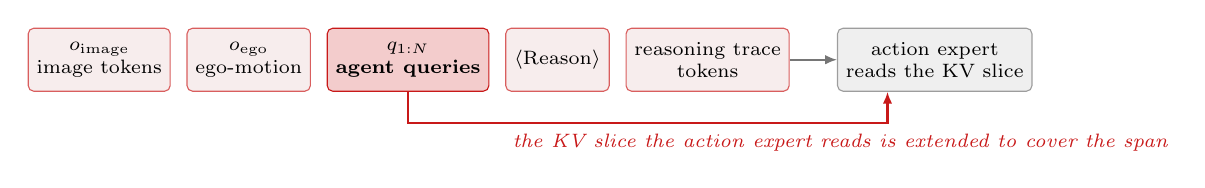
\begin{tikzpicture}[node distance=2mm]
    \node[nb,minimum height=8mm] (img)  {$o_{\text{image}}$\\image tokens};
    \node[nb,minimum height=8mm,right=of img] (ego) {$o_{\text{ego}}$\\ego-motion};
    \node[nbh,minimum height=8mm,right=of ego] (q) {$q_{1:N}$\\\alert{agent queries}};
    \node[nb,minimum height=8mm,right=of q] (rs) {$\langle\text{Reason}\rangle$};
    \node[nb,minimum height=8mm,right=of rs] (tr) {reasoning trace\\tokens};
    \node[nbg,minimum height=8mm,right=of tr,xshift=4mm] (ae) {action expert\\reads the KV slice};
    \draw[ar] (tr) -- (ae);
    \draw[arr] (q.south) -- ++(0,-4mm) -| ($(ae.south)+(-6mm,0)$)
      node[midway,below,font=\scriptsize\itshape,xshift=-6mm]
      {the KV slice the action expert reads is extended to cover the span};
  \end{tikzpicture}}
  \end{center}

  Agent queries are projected into the backbone embedding space and inserted
  \alert{before} the reasoning tokens. Causal attention then exposes every
  query to every reasoning token, so grounding reaches the language path and
  the control path at once.

  \vspace{0.3em}
  \begin{block}{The detection loss becomes the auxiliary objective AR1 asks for}
    Their future work\refcite{NVIDIA2025AlpamayoR1} suggests
    depth or scene-flow auxiliaries to improve the
    visual backbone. Supervising the span with a detection loss is a more
    targeted version of that idea, aimed at grounding the reasoning rather than
    at improving features in general.
  \end{block}
\end{frame}

\begin{frame}{Controls, because the span might simply be ignored}
  \small
  The dominant failure mode of an added input is that a model with an existing
  path to the answer learns to ignore the redundant one. Two ablations are
  built in from the start, not added afterwards.

  \vspace{0.7em}
  \begin{description}
    \item[Span masking] Replace the queries with learned null embeddings at
      inference and measure the change in the generated traces. No change means
      the span is inert.
    \item[Span corruption] Substitute queries taken from a different scene. A
      trace that adopts the foreign objects shows the span is genuinely read.
  \end{description}

  \vspace{0.6em}
  Attention mass placed on the query positions by the reasoning tokens is
  logged throughout as a continuous diagnostic, so the question is answered by
  a curve rather than by a single ablation number.

  \vspace{0.4em}
  $N$ is held in the tens and selected by decision relevance rather than raw
  confidence, and the token cost is reported alongside latency.
\end{frame}

\begin{frame}{Phase 3: temporal propagation, and the grounding reward}
  \small
  Queries are propagated between frames with ego-motion compensation rather
  than re-detected independently. Evaluation targets occlusion and
  reappearance, where the stateless variant cannot by construction retain an
  agent that has left the observation window.

  \vspace{0.5em}
  If time permits, the RL stage gains a \alert{grounding reward} analogous to
  AR1's reasoning-action consistency reward. Parse the trace into referenced
  categories, compare against the query set, score the match. Rule-based, so it
  needs neither new annotation nor a judge model.

  \vspace{0.4em}
  \begin{exampleblock}{Example}
    \footnotesize
    Trace: \emph{``yielding to the pedestrian on the right, lead vehicle
    stopped''}\\
    Referenced: \{pedestrian, vehicle\} \qquad
    Query set: \{car, car, truck\}\\
    Score: pedestrian unmatched, penalty applied.
  \end{exampleblock}

  \vspace{0.3em}
  \footnotesize
  This item is explicitly optional and is the first thing I drop if the
  schedule slips.
\end{frame}

\begin{frame}{Evaluation protocol and expected contributions}
  \footnotesize
  \textbf{Evaluation.}
  \begin{itemize}
    \item \emph{Grounding}: unsupported-reference rate per category and
      scenario, plus attention mass on the span.
    \item \emph{Open-loop}: minADE$_6$ and minFDE over 6.4\,s, nominal and
      long-tail splits separately, since the claimed benefit concentrates in
      the latter.
    \item \emph{Closed-loop}: close-encounter rate, off-road rate and AlpaSim
      score, with an occlusion breakdown.
    \item \emph{Cost}: added tokens, added parameters, end-to-end latency
      against the reported 99\,ms budget.
  \end{itemize}

  \vspace{0.3em}
  \textbf{Expected contributions.}
  \begin{enumerate}
    \item The first quantitative characterisation of object-level hallucination
      in a released driving VLA, with a reusable protocol. This stands
      regardless of H2 and H3.
    \item An architecture and training recipe for a sensor-grounded, temporally
      propagated object span, with ablations that establish whether it is read
      rather than ignored.
    \item A characterisation of the token-budget against grounding trade-off,
      directly relevant to embedded deployment.
    \item A workshop or conference submission, with code released against the
      public checkpoints.
  \end{enumerate}
  \vspace{-0.4em}
\end{frame}



% ============================================================================
\section{Connection}
% ============================================================================

\begin{frame}{How the stay builds on the thesis}
  The thesis produces exactly the representation AR1 lacks.

  \vspace{0.4em}
  \begin{columns}[T,onlytextwidth]
    \begin{column}{0.47\textwidth}
      \textbf{\color{tuered}The thesis delivers}
      \begin{itemize}
        \footnotesize
        \item A compact set of agent queries, tens rather than thousands.
        \item Grounded in sensor data by a detection loss.
        \item Carrying persistent identity across frames through a memory bank.
        \item Initialised from the data rather than from a constant.
      \end{itemize}
    \end{column}
    \begin{column}{0.47\textwidth}
      \textbf{\color{tuered}The stay requires}
      \begin{itemize}
        \footnotesize
        \item A span short enough to insert into a token sequence.
        \item A supervision signal that grounds it in the scene.
        \item State that survives beyond the observation window.
        \item Queries that reflect this scene, not a prior over scenes.
      \end{itemize}
    \end{column}
  \end{columns}

  \vspace{0.5em}
  \begin{block}{In one sentence}
    The thesis answers how to build the representation. The stay asks what a
    reasoning model does with it.
  \end{block}
\end{frame}

\begin{frame}{Scientific questions to be addressed during the stay}
  \begin{enumerate}
    \item How often does a released driving VLA refer to objects that are not
      there, measured against human-written traces on the same clips?
    \item Does conditioning the reasoning on an explicit, detection-supervised
      object span reduce that rate, and can the span be shown to be used rather
      than ignored?
    \item Does propagating the queries across frames extend the benefit to
      occlusion and reappearance, which causal locality and a per-frame
      KV-cache cannot reach?
    \item What does the span cost in tokens, parameters and latency, and is
      that affordable on automotive-grade embedded hardware?
    \item Can a rule-based grounding reward replace a judge model in the RL
      stage?
  \end{enumerate}
\end{frame}

\begin{frame}{Fit with the Mobile Perception Systems Lab}
  \begin{itemize}
    \item The lab's long-term goal is spatio-temporal reasoning that lets a
      mobile platform anticipate future events, identified as a bottleneck in
      crowded inner-city settings. \tueemph{H3 is a concrete instance of that
      problem.}
    \item The test vehicle carries a 360-degree camera setup with LiDAR and
      radar, which enables the multimodal variant where LiDAR-derived queries
      ground an otherwise camera-only backbone. \tueemph{My preliminary work is
      LiDAR-based and transfers directly.}
    \item Work in the lab on token-efficient vision transformers addresses
      precisely the cost an added span incurs, which the Phase 2 token-budget
      analysis measures.
    \item Radar perception suggests extending the multimodal variant to the
      conditions where a camera backbone is least reliable.
    \item Closed-loop evaluation would run in the TU/e digital twin alongside
      the public AlpaSim scenario sets.
  \end{itemize}
\end{frame}

\begin{frame}{Three things to take away}
  \begin{enumerate}
    \item \tueemph{A result.} Deriving agent queries from a LiDAR heatmap
      instead of a learned embedding more than doubles EPA and roughly halves
      minADE against a baseline I trained in the same harness, at an unchanged
      parameter count. Camera fusion adds to that rather than replacing it.
    \item \tueemph{A limitation I can explain.} Tracking lags because the
      classification score is well ranked but badly calibrated against a hard
      survival gate, and I can point to the measurement that shows it.
    \item \tueemph{A proposal that follows from both.} AR1 reasons about
      objects it has no grounded representation of. The thesis builds that
      representation. The stay measures whether supplying it makes the
      reasoning true and the driving safer.
  \end{enumerate}
\end{frame}

{
\setbeamercolor{background canvas}{bg=tuered}
\begin{frame}[plain]
  \vfill
  \centering
  {\color{white}\Huge\textbf{Thank you}}\\[1.0em]
  {\color{white}\large Technical discussion and questions}
  \vfill
\end{frame}
}

% ============================================================================
\appendix
% ============================================================================

% TODO:add visulizations

\begin{frame}{Backup: why EPA is the primary metric}
  \vspace{-0.3em}
  EPA as defined by ViP3D\refcite{Gu2023ViP3D}:
  \[
    \mathrm{EPA} = \max\!\left(0,\;
      \frac{N_{\text{hit}} - \alpha N_{FP}}{N_{\mathrm{GT}}}\right),
    \qquad \alpha = 0.5
  \]
  \begin{itemize}
    \item Predicted agents are matched to annotated agents by Hungarian
      assignment on centre distance, gated at 2\,m, in the current frame.
    \item $N_{\text{hit}}$ counts an agent as a hit only if its minFDE$_K$
      stays within 2\,m at the horizon.
    \item minADE, minFDE and MR average \alert{only over matched agents}, so a
      model that detects fewer objects can improve all three.
    \item $N_{\mathrm{GT}}$ counts the annotated agents that survive the whole
      horizon, and false positives are subtracted, so EPA penalises both
      failure modes at once.
  \end{itemize}
\end{frame}


\begin{frame}{Backup: the tracking interface}
  The model's inference behaviour is controlled by parameters that no gradient
  touches, because they sit behind hard comparisons and a top-$K$ selection.

  \vspace{0.4em}
  \begin{columns}[T,onlytextwidth]
    \begin{column}{0.46\textwidth}
      \footnotesize
      \begin{tabular}{ll}
        \toprule
        Parameter & Value \\
        \midrule
        confirm a new track   & 0.40 \\
        keep a track alive    & 0.35 \\
        miss tolerance        & 5 frames \\
        heatmap NMS kernel    & $3{\times}3$ \\
        active-track suppression & $5{\times}5$ cells \\
        queries $K$           & 300 \\
        \bottomrule
      \end{tabular}
    \end{column}
    \begin{column}{0.50\textwidth}
      \footnotesize
      True positives score $0.73 \pm 0.18$ and false positives
      $0.57 \pm 0.16$. The ranking is good, the absolute calibration is not.
      With that spread a confirmed track dips below the $0.35$ gate in
      roughly 17\,\% of frames, is deleted, and is reacquired under a new
      identity.

      \vspace{0.4em}
      This costs tracking metrics while leaving detection metrics largely
      intact, which is why AMOTA and EPA disagree.

      \vspace{0.4em}
      Any gain found by tuning these is free at inference. No retraining, no
      extra parameters.
    \end{column}
  \end{columns}
\end{frame}

\begin{frame}{Backup: batch size and query count sweep}
  \footnotesize
  Stage 1, LiDAR only, nuScenes validation. Learning rate was sqrt-scaled with
  the batch size.

  \vspace{0.4em}
  \begin{table}
    \centering
    \begin{tabular}{lccl}
      \toprule
      Stage-1 variant & minADE \dn & EPA \up & Note \\
      \midrule
      300 queries, effective batch 8  & 0.956 & 0.293 & best, the row in the results table \\
      300 queries, batch 16 & 0.997 & 0.277 & \\
      300 queries, batch 32 & 1.114 & 0.236 & \\
      300 queries, batch 64 & 1.061 & 0.256 & \\
      100 queries, batch 8  & 1.022 & 0.256 & \\
      100 queries, batch 16 & 1.528 & 0.234 & \\
      \bottomrule
    \end{tabular}
  \end{table}

  \vspace{0.4em}
  \normalsize
  Accuracy degrades close to monotonically with batch size even with the
  learning rate scaled, which is consistent with the usual small-batch-noise
  argument. I report it as an observation rather than an explanation, because
  the flat-minima claim is testable on the checkpoints I already have and I
  have not tested it yet.
\end{frame}

\begin{frame}{Backup: configuration details}
  \footnotesize
  \begin{columns}[T,onlytextwidth]
    \begin{column}{0.48\textwidth}
      \textbf{LiDAR branch}
      \begin{itemize}
        \item Point cloud range $\pm 51.2$\,m, pillars of $0.2$\,m,
          20 points per pillar.
        \item PillarFeatureNet $5 \to 64$, PointPillarsScatter to
          $512 \times 512$.
        \item SECOND with strides $[2,2]$, SECONDFPN to
          $384 \times 256 \times 256$, so $0.4$\,m per BEV cell.
        \item 10 accumulated sweeps, 5 features per point.
      \end{itemize}
      \textbf{Heatmap head}
      \begin{itemize}
        \item CenterPoint nuScenes task grouping, so pretrained per-task
          weights still line up.
        \item Gaussian focal loss, radius from the box footprint.
      \end{itemize}
    \end{column}
    \begin{column}{0.48\textwidth}
      \textbf{Decoder}
      \begin{itemize}
        \item Embedding 256, 8 heads, FFN 512, dropout 0.1.
        \item Layer 0 deformable BEV attention, 4 sampling points per query.
        \item Layer 1 SMCA over 4 FPN levels and 6 cameras, anisotropic
          $\sigma$ from the projected box size.
        \item Reference points and sizes updated after each layer, sizes
          detached after layer 0.
      \end{itemize}
      \textbf{Schedule}
      \begin{itemize}
        \item Stage 1: 20 epochs, camera path frozen.
        \item Stage 2: 6 epochs, LiDAR path frozen, lr $3.5\mathrm{e}{-4}$.
      \end{itemize}
    \end{column}
  \end{columns}
\end{frame}

\begin{frame}{Backup: questions for the lab}
  \begin{enumerate}
    \item Which AR1 checkpoints and which parts of the Alpamayo training stack
      are available inside the lab, and is AlpaSim usable for closed-loop
      evaluation in February?
    \item Do the campus recordings carry 3D annotations, or would Phase 1 run
      on the public clips and the campus data enter only in Phase 2 and 3?
    \item What compute would a fine-tuning run have, and how is it scheduled?
    \item Is the LiDAR and radar on the test vehicle time-synchronised and
      calibrated against the 360-degree camera rig to the accuracy that
      query-level projection needs?
    \item Who else in the group works on the reasoning side, and would this sit
      alongside an existing effort or beside it?
    \item What is a realistic publication target for a four-month result in
      your experience?
  \end{enumerate}
\end{frame}

% ----------------------------------------------------------------------------
%  References.  Entries come from the thesis bibliography, copied to
%  bib/references.bib, plus the Alpamayo-R1 entry added at the end of it.
% ----------------------------------------------------------------------------
\begin{frame}[allowframebreaks]{References}
  \printbibliography[heading=none]
\end{frame}

\end{document}
